% !Mode:: "TeX:UTF-8" 

\BiChapter{基于贝叶斯网络的克隆创建时一致性维护需求预测方法}
{Predicting Clone Consistency-Requirement Based on Bayesian Network at Clone Cloning Time}

\BiSection{引言}
{Introduction}

由于日益增长的软件开发的需求,开发人员在软件开发过程中通过复制粘贴既有代码(称为克隆创建),向系统中引入新的克隆代码。新产生的克隆代码会随着系统演化,其演化过程中可能会发生一致性变化。然而,克隆代码的一致性变化不仅会导致系统额外的维护代价,遗忘该一致性变化还会引入与之相关的克隆一致性缺陷,从而将进一步增大系统的维护代价。本文将由复制粘贴操作创建的克隆代码在其演化过程中所发生的一致性变化,称为克隆代码创建时的一致性维护需求。在克隆代码创建时预测克隆代码的一致性维护需求,可以帮助降低系统的维护代价,从而帮助提高软件质量和可维护性。

鉴于此,在定义克隆代码创建时的一致性变化和一致性维护需求的基础上,本章使用机器学习中的贝叶斯网络方法在克隆代码创建时预测其一致性维护需求。为训练克隆代码创建时一致性预测模型,首先通过构建软件系统的克隆家系来收集系统中所有的克隆创建实例(复制粘贴导致的克隆代码)。然后,提取了代码属性和上下文属性两组属性值表示克隆代码创建实例。最后,使用贝叶斯网络方法训练机器学习模型,并预测克隆代码创建时的一致性维护需求。在四个开源软件系统上对本章方法进行了评估,实验结果表明本章方法以较高的准确率和召回率高效地预测克隆代码创建时的一致性维护需求。本章所提出的预测方法可以帮助程序开发员在克隆代码创建时预测克隆代码的一致性,降低克隆代码导致的额外的维护代价,从而提高软件的质量和可维护性。

\BiSection{克隆代码创建时一致性维护需求}
{Clone Cloning Consistency-Requirement}

\BiSubsection{相关研究}
{Related Work}

在软件开发过程中,通过复制和粘贴操作复用既有代码已经成为一种常见的软件开发手段\cite{koschke2007survey}。复制粘贴活动可以减少软件开发时间和提高软件开发效率,但同时也会向软件系统中创建新的克隆代码(克隆创建)。克隆代码会长时间的存在于软件系统中,并同时随着软件系统进行演化。克隆代码随系统进行演化的过程可以使用克隆家系进行描述\cite{kim2005empirical}(克隆演化见本文~\ref{ref-evolution}~节)。经研究发现在克隆代码的演化过程中,克隆组内的某一克隆代码片段可能会被程序开发人员修改,从而引发克隆代码的变化。同时,由于同组的克隆代码彼此相似,这种变化也可能会传播到同组的其它克隆代码片段中,从而引起克隆组一致性变化\cite{saha2011automatic}。

为了帮助分析克隆代码的变化以及演化情况,本文第二章基于机器学习中的聚类方法挖掘克隆代码的演化特征。研究表明在克隆代码的演化过程中,存在相当数量的克隆代码会发生变化。这些发生变化的克隆代码也会引发克隆组的一致性变化模式。更为重要的是,演化中的克隆代码的一致性变化往往多于不一致性变化,因此在第二章中本文建议程序开发人员需要警惕克隆变化,并且当发生变化时需要考虑克隆代码的一致性问题。(具体可参考本文~\ref{ref-characteristics}~节)

为确保演化中的克隆代码的一致性,程序开发人员需要对发生变化的克隆进行一致性维护,从而导致额外的维护代价。而遗忘克隆的一致性变化,会导致克隆代码的不一致缺陷,从而进一步增加软件的维护代价\cite{aversano2007clones}\cite{bettenburg2009empirical}。本文将在演化过程中由于克隆一致性变化所导致的维护代价称为一致性维护代价。为了避免克隆代码的一致性维护代价,程序开发人员可以在复制粘贴时避免可能发生一致性变化的克隆代码,或者仅允许不会发生一致性变化的克隆代码的产生。换言之,在复制粘贴时预测克隆代码在演化过程中是否会发生一致性变化,可帮助避免一致性维护代价。

因此,Wang等人基于贝叶斯网络在复制粘贴时对克隆代码进行一致性维护需求预测,帮助避免需要一致性维护的克隆代码\cite{wang2012can}\cite{wang2014predicting}。该方法中提取了历史属性、代码属性和上下文属性三组属性表示复制粘贴操作,并使用贝叶斯网络预测克隆代码一致性维护需求。但是,该方法存在以下不足之处:
\begin{itemize}
\item
首先,所使用的历史属性与复制粘贴操作的关联性较弱,仅表示其所在文件的历史变化情况。同时历史属性的提取也增加了方法本身的困难程度(历史属性提取需要分析软件全部版本源代码);
\item
其次,所提取的代码属性和上下文属性不够充分,并不能完全的表示复制粘贴操作所导致的克隆代码。例如,代码属性中仅考虑了克隆代码与系统其它模块的调用和访问关系,并没有详细的考察克隆代码自身的一些属性特征。
\item
最后,方法中没有清晰的给出克隆变化以及一致性维护需求的定义。
\end{itemize}

鉴于此,本章对复制粘贴产生的克隆代码的一致性维护需求,进行了进一步的深入研究。本章在克隆代码演化的基础上结合克隆代码一致性维护,首先给出了一种克隆代码一致性变化以及一致性维护需求的定义,可更为准确地帮助预测克隆的一致性维护需求。然后,本文在Wang等人研究的基础上,改进了克隆代码一致性维护需求预测所使用的度量值。舍弃了与复制粘贴操作关联性不强的历史属性,并进一步扩展了代码属性和上下文属性,可以更为详细和细致的表示由复制粘贴操作导致的克隆代码。最后,使用贝叶斯网络在克隆代码创建时预测其一致性维护需求。本章方法可以帮助程序开发人员降低克隆代码的一致性维护代价,避免克隆一致性缺陷。
%因此,本章方法可可以提高系统的可维护性和软件质量。




%上述不足限制了该方法的实际应用,无法将其应用到具体的软件开发实践中。为解决上述问题,本文对由于复制粘贴产生的克隆代码的一致性维护需求预测进行了进一步研究,在软件开发过程中实现对其的一致性维护需求预测。首先,本文给出新的一致性变化定义,可更为准确地定义和预测克隆的一致性维护需求。然后,在通过构建克隆家系提取复制和粘贴操作后,舍弃历史属性并扩展了代码属性和上下文属性用于表示复制和粘贴操作。然后,本文除使用贝叶斯网络作为预测模型之外,还分析了其它预测模型在克隆代码一致性需求预测问题上的适用性。
%在预测克隆代码的一致性维护需求时,本文有保守模式和激进模式两种使用模式。使用保守模式开发人员可以谨慎的开发软件,通过仅允许不需要一致性维护的复制粘贴操作,从而避免引入会导致额外的克隆代码产生。使用激进模式下开发人员可以快速地开发软件节约开发时间,通过仅阻止需要一致性维护的复制粘贴操作,从而让软件开发人员安全快速的开发软件。本文使用不同的分类器在四个开源软件上进行了实验评估,结果表明本文方法可以同时在保守模式和激进模式下以较高的准确率和召回率对克隆代码进行一致性维护需求预测。本文的主要贡献如下:
%(1)本文定义了新的克隆代码一致性变,并根据其定义了克隆代码的一致性维护需求,可以更为准确的标识克隆代码的一致性维护代价;
%(2)本文使用并扩展代码属性和上下文属性两组属性组,实验结果表明所使用的属性在克隆一致性维护需求的预测中起到了积极的作用;
%(3)本文预测克隆代码的一致性维护需求,不仅在贝叶斯网络分类器上进行了实验评估,还在一般分类器上进行了实验验证,实验结果表明本文方法具有一般性,可以适用于一般的机器学习方法。


%%。本文使用NiCad检测克隆代码(包含Type 1、Type 2和Type 3克隆代码),并使用 {\em Unique Percentage Items (UPI)}来计算克隆片段之间的相似度\cite{roy2008nicad}。



\BiSubsection{克隆创建时一致性维护需求定义}
{The Definitions for Clone Cloning Consistency-Requirement}

在克隆代码的演化过程中,克隆片段可能会被开发人员修改,从而导致克隆代码的一致性变化,这种变化可能会导致额外的维护代价。为了描述这种克隆代码的修改,本章给出克隆代码变化时一致性变化定义,如下所示:\\

\begin{definition}
[创建时一致性变化(Changing Consistent Change)]  
\label{def-cloningchange}
给定两个克隆代码片段 $CF_1$和 $CF_2$,且它们被分别地修改为$CF'_1$和$CF'_2$。如果克隆代码$CF_1$和$CF_2$的变化满足以下条件,称此变化为{克隆创建时的一致性变化(Cloning Consistent Change)} , 
  \[
  \begin{array}[t]{cr}
    \mathit{textSim}(CF_i, CF'_i) < 1 & \forall i \in \{1,2\}  \\
  \end{array}
  \]
\end{definition}

%定义2.克隆变化.在版本$V_j$中存在某一克隆组$CG$, $CF$是$G$中某一克隆片段。当克隆演化到$V_{j+1}$版本时,$CF$在中仍存在该克隆组内,记为$CF'$。本文使用$SimText(CF,CF')$表示克隆片段是否发生变化:若$SimText(CF,CF')<1$,则克隆片段发生变化;若$SimText(CF,CF')=1$,则克隆片段未发生变化。其中$SimText(CF,CF')$计算方法与NiCad相同,使用$UPI$计算其相似度。

注意$\mathit {textSim}(CF_i, CF'_i)= 1 - UPI(CF_i, CF'_i)$,UPI是两个代码片段之间不同的代码行数占总代码行的比例。假如给定两个代码片段$CF_1$和$CF_2$,其$UPI(CF_1,CF_2)=0.3$表示两者的差异程度为30\%。同时,其相似度可根据$UPI$计算:$SimText (CF_1,CF_2)=1-UPI=0.7$,表示两者的相似度为70\%。本文在检测克隆代码时,设置克隆代码的相似度阈值为0.7,即相似度大于阈值的代码片段为克隆代码。该定义仅要求克隆代码片段 $ CF_1 $和$CF_2 $被同时修改。

创建时一致性变化,仅要求克隆代码片段被同时的修改。原因在于:在克隆代码创建时,目标是避免新创建的克隆代码在其未来演化过程中的一致性变化,及其所导致额外的维护代价。因此,只要两个克隆片段在其演化过程同时变化,即认为会导致额外维护代价。

克隆创建(复制粘贴操作)所导致的克隆组,会随着系统的演化而演化。在此过程中,组内克隆片段的变化也导致了克隆组的变化,并使用克隆演化模式描述克隆组的变化,称其为一致性变化模式或不一致变化模式。克隆组一致性变化模式定义如下所示:\\
\begin{definition}
[创建时一致性变化模式( Cloning Consistent Change Pattern)] 
\label{def-cloningpattern}
在软件版本 $j+1$中存在一个克隆组$CG'$ ,假设克隆组内至少存在两个克隆代码片段$CF'_1$ 和 $CF'_2$可以与映射到上一版本$j$的克隆组$CG$中,且 $CG$中与之对应的克隆代码片段的 $(CF_1,CF_2)$被修改为$(CF'_1,CF'_2)$。如果克隆片段之间的变化( $(CF_1,CF_2)$变化至$(CF'_1,CF'_2)$满足克隆片段的“一致性变化(Consistent Change)”,则称克隆组$CG'$具有一致性变化模式(Consistent Change Pattern)。
\end{definition}

%定义3.一致性变化模式.克隆组$CG$从版本$V_j$到$V_j+1$演化为$CG'$。假如$CG$中至少存在两个克隆代码片段$(CF_1,CF_2)$同时发生了变化,记为$(CF'_1,CF'_2)$。如果$CF'_1$和$CF'_2$同时满足$SimText(CF_1,CF'_1)<1$且$SimText(CF_2,CF'_2)<1$,称克隆组$CG$在演化为$CG'$时发生一致性变化模式,反之称为不一致变化模式。

本章定义的克隆创建时的一致性变化模式,与其它论文中的定义不同。其原因在于:本章目的在于预测克隆代码的一致性所引发的维护代价。为了便于读者更容易理解克隆创建的克隆组的一致性维护需求,本章现给出克隆创建实例的定义,如下所示:\\

\begin{definition}
[克隆创建实例( Clone Cloning Instance)] 
\label{def-cloninginstance}
克隆创建实例:软件版本 $j$中的一个克隆组$CG$是克隆创建实例,如果该克隆组$CG$是其克隆家系$CGE$的根节点。
\end{definition}
%In the above definitions, we identify a $CG$ created by a cloning operation (copy and paste) as a new $CGE$ root that begins its evolution. 

%定义1.复制粘贴实例.给定一个克隆组$CG$,其整个演化历史可用克隆家系表示。在表示克隆组$CG$整个演化历史的克隆家系中,第一次出现的克隆组是认为是由复制粘贴活动导致,并称第一次出现的克隆组为复制粘贴实例。


给定一个克隆创建实例所产生的克隆组,在其演化过程中,可能会发生一致性变化模式。克隆组的一致性变化会引发一致性维护代价,从而降低软件质量。因此,在克隆创建时,预测其在演化过程是否会发生一致性变化,可以避免与克隆创建导致的克隆代码的一致性维护代价。本文将创建时克隆代码导致的一致性变化,称为克隆一致性维护需求。克隆创建时的一致性维护需求定义如下:\\

\begin{definition}
[创建时一致性维护需求(Cloning Consistency-Requirement)] 
 \label{def-cloningrequirement}
给定版本 $j$中一个克隆创建实例,$CG$满足克隆一致性维护需求(Consistency-Requirement),如果在版本$k$中存在一个克隆实例 $CG'$($k>j$)满足以下条件: (1) 在$CG'$中至少存在两个克隆片段在其克隆家系$CGE$中可以映射到克隆实例 $CG$中, (2) $CG'$ 具有“一致性变化模式”(Consistent Change Pattern)。反之,假如克隆创建实例$CG$ 不满足克隆一致性维护需求条件,称该克隆实例不需要一致性维护(Consistency-Requirement Free,或者Consistency-Free)。
\end{definition}

%定义4.一致性维护需求.给定一个复制粘贴实例(即克隆组),可以用克隆家系描述其整个演化过程。在其演化过程中,该复制粘贴实例至少发生过一次一致性变化模式,则称该实例满足一致性维护需求。

最终,可以将本章的的研究问题表述如下:给定一个克隆创建实例$CG$,即复制粘贴活动导致的克隆代码,预测创建实例$CG$是否满足克隆创建时的一致性维护需求。

更进一步,根据上述定义克隆创建实例只有两种状态:满足和不满足一致性维护需求。本章克隆创建时的克隆一致性需求预测问题可转换为一个典型的分类问题,因此使用机器学习模型解决此分类问题,具体方法见下文。

\BiSection{克隆代码创建时一致性维护需求预测框架}
{The Framework of Clone Cloning Consistency-Requirement Prediction }

为解决本章所提出的克隆一致性需求维护预测问题,本文首先给出了一个方法框架。
基于贝叶斯网络的克隆创建时一致性维护需求预测框架如图~\ref{framwork3}所示。
方法可以划分为三个阶段,克隆创建实例收集阶段、克隆创建实例表示阶段和一致性维护需求预测阶段。收集阶段旨在收集系统中全部的克隆创建实例,可将其用于使用机器学习方法中来训练预测模型。由于实际的克隆创建实例无法直接应用于机器学习方法中,因此在表示步骤中将提取相应的属性值表示克隆创建实例。接下来,在预测步骤,使用属性化的克隆创建实例构建和训练机器学习模型,并使用其预测克隆创建实例的克隆一致性维护需求。

\begin{figure}[htbp]
\centering
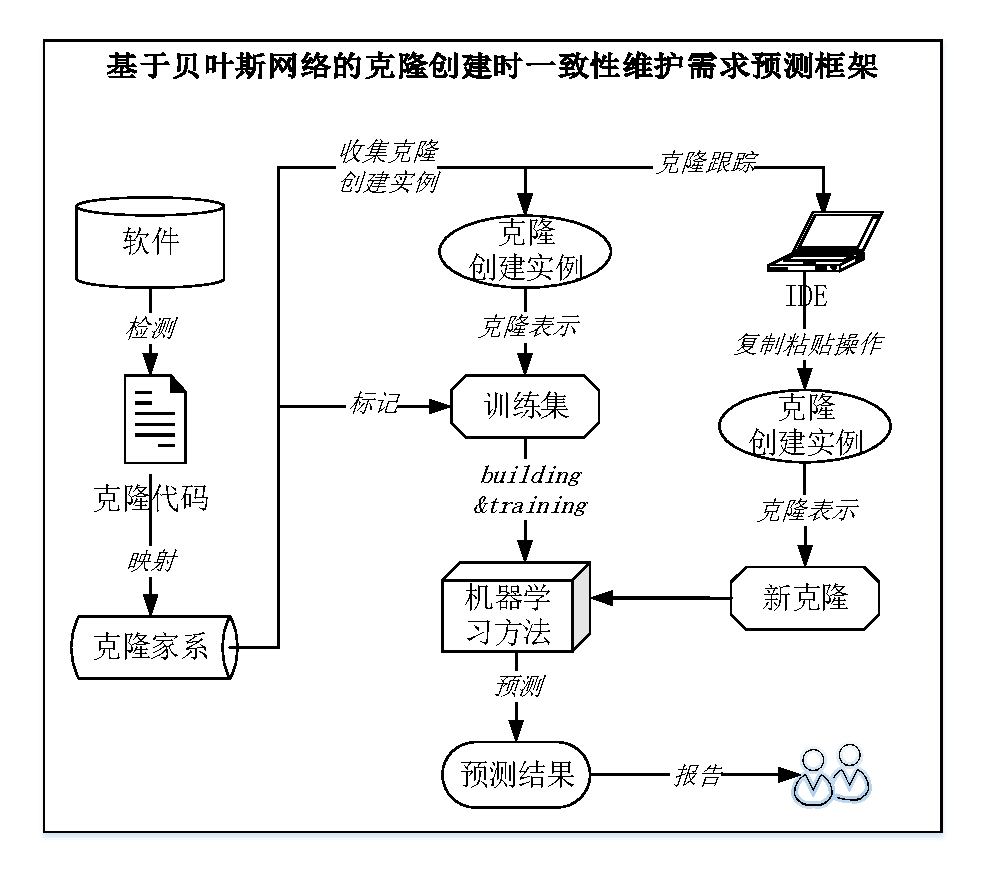
\includegraphics[width = 0.8\textwidth]{framework3.pdf}
\bicaption[framwork3]{}
{基于贝叶斯网络的克隆创建时一致性维护需求预测框架}
{Fig.$\!$}{The framework for clone cloning consistency prediction based on Bayesian network}
\vspace{-1em}
\end{figure}

具体来说,在收集阶段中,通过构建系统的克隆家系从软件中收集所有的克隆创建实例。使用NiCad来检测软件版本中的所有克隆,并通过在相邻版本的克隆组之间进行映射来构建克隆家系,用于识别克隆创建实例。在表示阶段中,通过提取属性值表示克隆创建实例,提取了代码属性、上下文属性两组组属性组分别表被复制和粘贴的克隆代码。在预测阶段中,使用收集到的克隆创建实例训练贝叶斯网络,并在克隆创建时预测克隆一致性维护需求。在使用已构建好的模型进行预测时,可将该模型嵌入到软件开发环境中。软件开发环境需要实时监测复制粘贴操作(克隆创建实例),然后提取克隆创建实例的度量值。最后,使用模型预测其一致性维护需求,根据预测结果提醒程序开发人员采取进一步的操作。

克隆创建实例有两种不同的预测结果,即满足一致性维护需求和不满足维护需求。
对于满足一致性维护需求实例来说,其在将来的演化中可能会引发一致性变化,程序开发人员可以根据情况选择拒绝此变化实例。对于不满足一致性维护需求实例来说,其在将来的演化中不会引发一致性变化,程序开发人员可以根据情况选择接受此变化实例。

本章基于贝叶斯网络预测克隆创建实例的一致性。使用克隆创建实例的属性表示贝叶斯网络中的节点,并用于构造贝叶斯网络的结构。使用收集到的克隆创建实例学习贝叶斯网络的参数,从而完成模型的训练,细节可参考本文后续章节。

\BiSection{收集克隆创建实例}
{Collecting Clone Cloning Instance}
\label{lab-checkcopied}
收集克隆创建实例的目的在于生成克隆一致性预测的训练集,并将其用于训练机器学习模型。通过构建系统的克隆家系并识别其中的克隆演化模式,可以从软件中收集所有的克隆创建实例。首先使用NiCad来检测软件版本中的所有克隆,然后通过在相邻版本的克隆组之间进行映射来构建克隆家系,最后识别克隆一致性演化模式识别系统中的克隆创建实例。

根据定义~\ref{def-cloninginstance}~,本文假定克隆家系$CGE$中第一次出现的克隆代码是由复制粘贴操作导致的,即是克隆创建实例。因此,通过检测系统的克隆代码并构建克隆家系,可以完成对克隆创建实例的收集。

(1)构建克隆家系。首先,下载系统所有版本的源代码,并使用NiCad的默认配置检测检测每一版本的中Type1-3的克隆代码。然后,通过映射所有相邻版本的克隆代码,构建系统中全部克隆家系。为完成版本间的映射,为每个克隆片段生成一个克隆区域描述符 $CRD$\cite{duala2010clone},使用基于$CRD$的克隆映射算法映射两个连续版本之间的所有克隆片段和克隆组\cite{ci2013new}\cite{ci2013newD}。根据克隆映射结果,构建系统的克隆家系。

(2)收集克隆创建实例并标识一致性维护需求。克隆家系是克隆演化的有向无环图,图中根节点是由复制粘贴操导致的克隆创建实例。因此,根据定义~\ref{def-cloninginstance}~通过遍历克隆家系的根节点,可收集系统中所有的克隆创建实例。在收集克隆创建实例的时候,同时根据定义~\ref{def-cloningchange}~和~\ref{def-cloningpattern}~识别克隆一致性变化模式,从而确定克隆创建实例在其未来演化过程发生的一致性变化。根据定义~\ref{def-cloningrequirement}~,如果克隆创建实例在其演化过程中发生了一致性变化模式(~\ref{def-cloningpattern}~),则该实例满足一致性维护需求,否则不满足维护需求。

(3)确认复制和粘贴代码。在收集克隆变化实例后,还需确认该实例中的被复制和被粘贴代码。由于被复制代码会较早地存在软件中,可将创建实例中的克隆代码向上一软件版本中进行映射。假定被复制代码会应存在于上一版本中,被粘贴代码不存在上版本中。根据映射结果,可能会存在两种情况:(a)其中一个克隆代码可以映射,另一个未映射。认为映射代码为被复制代码,未映射为被粘贴代码。(b)两者均没有映射。此情况下随机选取一个为被复制代码,另一个未未被粘贴代码。原因是两者互为克隆代码,彼此之间相似,故随机选取一个为被复制代码并不影响预测结果。注意不存在两者均可映射的情况,应在上一版本检测为克隆代码。\footnote{幸运的是,大多数克隆组只有两个克隆片段,所以这个决定不会影响我们的克隆预测。对于具有多个克隆片段的克隆组,则随机选取两个作为克隆创建实例。}

\BiSection{克隆创建实例表示}
{Representation of Clone Cloning Instance}

%由于实际的克隆创建实例无法直接应用于机器学习方法中,因此在表示步骤中将提取相应的属性值表示克隆创建实例。在表示阶段中,通过提取属性值表示克隆创建实例,提取了代码属性、上下文属性两组组属性组分别表被复制和粘贴的克隆代码。

为使用机器学习方法预测复制粘贴实例的一致性维护需求,本文分别提取了两组属性特征表示复制粘贴实例:代码属性和上下文属性。

代码属性是被复制代码的属性,从代码自身角度表示被复制代码,描述被复制代码的词法和语法信息。部分代码属性源于Wang的工作,本文在其基础上进行了扩展,新增Halstead度量属性、结构属性等。Halstead属性经常用于软件预测中,是用于描述代码特征的度量。结构属性是从代码的语法结构信息。具体的代码属性如下所示:
\begin{itemize}
\item 克隆粒度:被复制代码的规模,使用代码行数表示。
\item Halstead度量:被复制代码的代码复杂度,有四个度量值,分别为操作符种类、操作数种类、操作符总量、操作数总量。
\item  结构属性:被复制代码的结构特征,包括if\_then, if\_else, switch, while, do, for, assignment, this\_or\_super等语句的统计。
\item  参数访问数量:被复制代码中所有函数的参数访问数量统计。
\item  总函数调用:被复制代码中所有函数调用的次数统计。
\item  本地函数调用:被复制的代码中,调用函数与被复制片段在相同类的调用次数统计。
\item  库函数调用:被复制的代码中,库函数的调用次数统计,包括java库函数的调用、eclipse库函数的调用以及第三方包函数的调用。
\item  其它调用:被复制的代码中,既不是库函数调用、也不是本地函数调用的其它调用次数统计,如同项目内其它包函数调用、或同包内其它类中的函数调用。
\end{itemize}

上下文属性是被复制和被粘贴代码之间的关系属性,表示两者之间的克隆关系。部分上下文属性来自Wang的工作,同时本文也进行了扩展,新增代码相似度、参数类型相似度和块信息标识等属性。具体的上下文属性如下所示:
\begin{itemize}
\item 	代码相似度:被复制与被粘贴的代码的相似度,使用和NiCad相同的方式计算。
\item 	局部克隆标识:被复制及粘贴的代码片段是否在同一个文件中。
\item 	文件名相似度:被复制和被粘贴代码所在文件的名相似度。假定文件名分别为$M_1$和$M_2$,则文件名相似度为$Sim(M_1,M_2)$,采用李氏距离\cite{levenshtein1966binary}计算(剩余度量中相似度采用相同方法计算)。
\item 	文件名相似度变量:当克隆是局部克隆时,其文件名相似度为1,为非局部克隆时为0。该属性决定文件名相似度是否起效。
\item 	方法名相似度:被复制和被粘贴代码所在方法的方法名字相似度。
\item 	总参数名相似度:假定被复制和被粘贴代码所在方法为$M$和$N$,计算其参数名相似度之和。假设M和N分别包含m和n个参数,即$(P_1,P_2,…,P_m)$和$(Q_1,Q_2,…,Q_n)$,则该度量值为$Sum(Sim(P_i,Q_j))$。
\item 	最大参数名相似度:假定被复制和被粘贴代码所在方法为M和N,其大参数名相似度。假设M和N分别包含m和n个参数,即$(P_1,P_2,…,P_m)$和$(Q_1,Q_2,…,Q_n)$,该度量值为$Max(Sim(P_i,Q_j))$。
\item 	总参数类型相似度:被复制和被粘贴代码所在方法分别为$M$和$N$,其参数类型相似度之和。假设$M$和$N$分别包含$m$和$n$个参数,其参数类型分别为$(P_1,P_2,…,P_m)$和$(Q_1,Q_2,…,Q_n)$,该度量值为$Sum(Sim(P_i,Q_j))$。
\item 	块信息标识:被复制和被粘贴代码的上下文信息是否相同,相同为1,反之为0。
\end{itemize}

\BiSection{贝叶斯网络}
{Bayesian Network}

本节使用贝叶斯网络方法对复制粘贴实例进行一致性需求维护。贝叶斯网络是一种概率模型,使用已经发生的事件预测将来可能发生的事件\cite{friedman1997bayesian}。贝叶斯网络模型的生成和训练均使用开源软件工具WEKA。将复制粘贴实例划分为训练集和测试集,使用训练集训练贝叶斯网络生成预测模型,使用K2搜索算法建立网络结构,并设置贝叶斯网络最大父节点个数为3。使用测试集评估贝叶斯网络的预测能力,贝叶斯网络会计算每一个复制粘贴实例的概率值,表示该实例需要一致性维护需求的概率(在0~1之间,数值接近于1表示需要一致性维护,接近于0表示不需要一致性维护)。

\BiSection{预测阶段}
{Predicting}

%接下来,在预测步骤,使用属性化的克隆创建实例构建和训练机器学习模型,并使用其预测克隆创建实例的克隆一致性维护需求。在预测阶段中,使用收集到的克隆创建实例训练贝叶斯网络,并在克隆创建时预测克隆一致性维护需求。在使用已构建好的模型进行预测时,可将该模型嵌入到软件开发环境中。软件开发环境需要实时监测复制粘贴操作(克隆创建实例),然后提取克隆创建实例的度量值。最后,使用模型预测其一致性维护需求,根据预测结果提醒程序开发人员采取进一步的操作。

\BiSubsection{模型训练与预测}
{Training and Predicting}

提取复制粘贴实例的属性特征后,可进行构建和训练预测模型。本文所采用的机器学习方法为有监督学习方法,因此为还需确认复制粘贴实例的一致性维护需求状态。根据定义4的描述,标记实例的一致性维护需求状态。复制粘贴实例的一致性维护需求状态仅有两种情况:需要一致性维护和不需要一致性维护。为标记其维护状态,可通过遍历克隆家系的演化情况,根据定义4进行标记。通标记维护状态,获得了模型训练的训练数据集,可构建和训练一致性维护需求的预测器。


在预测阶段,一致性维护需求预测可和软件开发过程相结合。将训练好的模型嵌入到软件开发环境(如eclipse)中,在复制粘贴时进行预测。需在软件开发环境中监测复制粘贴操作,并使用训练好的预测器对其进行一致性维护需求预测。本文方法可方便的集成于软件开发环境中,如eclipse的插件。在软件开发过程中帮助程序开发人员在预测由复制粘贴产生的克隆代码的一致性维护需求。首先,在软件开发环境中需监测程序员的复制和粘贴操作,识别由此产生的克隆代码。然后,根据上文描述的代码和上下文特征,提取相应的特征表示该复制和粘贴操作。最后,使用训练好的预测器预测该复制粘贴实例的一致性维护需求,将预测器给出的预测结果通知程序开发人员进一步进行处理。

\BiSubsection{使用模式}
{Predicting}

复制粘贴操作有两种状态,分别为需要一致性维护和不需要一致性维护。在使用本文方法进行一致性维护需求预测时,本文可以有两种不同的使用模式,即保守模式和激进模式。

\begin{itemize}
\item 
保守模式:面向不需要一致性维护的复制粘贴实例。在保守模式下,程序员比较谨慎的执行复制和粘贴操作,仅仅允许不需要一致性维护需求的实例的发生,并且会尽量阻止需要一致性维护需求的实例,从而尽量避免引入额外的维护代价。
\item
激进模式:面向需要一致性维护需求的复制粘贴实例。在激进模式下,尽量避免需要一致性维护需求的实例,同时尽量允许不需要一致性维护需求的实例产生,从而节约开发时间。
\end{itemize}

两种不同使用模式可以给程序开发人员不同的选择,从而以适用于不同开发场景。保守模式下允许不需要一致性维护需要的复制粘贴实例,可让程序开发人员更加安全的开发程序,从而避免可能的缺陷。激进模式下阻止需要一致性维护的复制粘贴实例,可尽可能的复用现有的程序,让程序开发人员更加快速的开发程序。在实际的使用中,程序人员可根据不同的需求选择使用相应模式。

\BiSection{实验结果与分析}
{Experiment Results and Analysis}

\BiSubsection{实验设置}
{Experiment Step}

为评估本文方法,本文选取了四个开源软件进行实验。实验系统的基本信息如表1所示,给出4个实验系统的复制粘贴实例的统计信息。从表~\ref{cpsta}~中可看出,软件系统中存在大量的复制粘贴实例,数量从633到3366。同时软件系统中的大多数复制粘贴实例不需要一致性维护(比例从59.8\%到88.47\%)。但是软件系统中也存在较多数量的需要一致性维护的复制粘贴实例(数量从73个到1353个)。

\begin{table}[htbp]
\bicaption[cpsta]{}{实验系统统计信息}
{Table$\!$}{Information of ...}
\vspace{0.5em}
\centering
\wuhao
\begin{tabular}{cccc}
\toprule[1.5pt]
\multirow{3}{*}{\textbf{Project}}& \multicolumn{2}{c}{\textbf{Number (Percentage) of Change Instances}} & \multirow{3}{*}{\textbf{Total}}\\
\cline{2-3}
&\textbf{Consistency-} &\textbf{Meeting} &  \\
&\textbf{Requirement Free}&\textbf{Consistency-Requirement}& \\
\midrule[1pt]
ArgoUML&	2574(77.07\%)&	766(22.93\%)&	3340\\
JEdit&	560(88.47\%)&	73(11.53\%)&	633\\
JFreeChart&	2013(59.80\%)&	1353(40.20\%)&	3366\\
Tuxguitar&	1016(71.10\%)&	413(28.90\%)&	1429\\
\bottomrule[1.5pt]
\end{tabular}
\end{table}

%%本文研究问题是复制粘贴实例的分类问题,采用机器学习方法解决该问题。机器学习领域中有较多的分类方法可以解决分类问题,如贝叶斯方法、决策树方法。本文分别使用贝叶斯网络分类器和其它的分类器进行实验。在贝叶斯网络实验中,预测方法为贝叶斯网络,并从三个不同的角度对本文方法进行全面评估。在分类器评估中,本文分别选取了几种不同的分类器,包括贝叶斯网络、朴素贝叶斯、决策树和决策树森林分类器,验证本文方法一般分类器上的预测能力。

贝叶斯网络实验可以分为全属性实验、属性组实验和交叉验证实验三个部分。全属性实验室采用所有的度量在所有系统上进行实验,用于评估本文方法的能力。属性组实验分析不同属性组对实验结果的影响。交叉验证实验使用训练好的模型去预测新系统,从而探索将本文模型在应用到新系统的预测能力。全属性实验和属性组实验在数据集上使用十倍交叉验证,交叉验证实验将不同的系统划分为训练集和测试集。本文有两种使用模式,在不同的模式下的目标不同,因此设置不同阈值进行实验分析。在保守模式下,面向不需要一致性维护的实例,其贝叶斯预测值较小(接近于0),选取阈值为0.01、0.05、0.10、0.15和0.20,当预测值小于等于给定阈值时认定该实例不需要一致性维护需求。在激进模式下,面向需要一致性维护的实例,其贝叶斯网络预测值较大(接近于1),选取阈值为0.5、1.6、0.7、0.8和0.9,当预测值大于等于该阈值认定该实例需要一致性维护。

由于复制粘贴操作有两种状态,即需要和不需要一致性维护,因此本文同样有两种使用模式与之对应(保守模式和激进模式)。在不同的模式下分别使用三种指标度量评估本文方法的预测能力。


\BiSubsection{保守模式实验}
{Conservative Scenario Experiment}


在保守模式下,对不需要一致性维护需求的复制粘贴实例进行评估。仅允许不需要一致性维护操作,从而防止导致额外维护代价。使用三个度量评估该使用模式:推荐率、准确率和召回率。
\begin{itemize}
\item	推荐率(Recommendation Rate,RR):指的是所推荐的不需要一致性维护的复制粘贴实例,即预测为不需要一致性维护的复制粘贴实例与系统中全部实例的比值。
\item  准确率(Precision,P):指所推荐的不需要一致性维护复制粘贴实例的准确率,即在预测为不需要一致性维护的复制粘贴实例中,正确预测的实例与所预测实例的比值。
\item  召回率(Recall,R):指所推荐的不需要一致性维护的复制粘贴实例的查全率,即预测为不需要一致性维护的复制粘贴实例,与系统中的不需要一致性维护的实例的比值。
\end{itemize}

\BiSubsubsection{全属性实验}
{Effectiveness Experiment}

全属性实验使用全部属性在四个实验系统上进行评估,实验结果如表~\ref{copyall0}所示(其中阈值Threshold简写为T)。由表中可以看出,本文方法在保守模式下均取得了较好效果,四个系统在不同的阈值的准确度较高(介于86.6~97.22\%),同时召回率也达到较高值(介于76.97~96.39\%)本文方法在使用全属性在贝叶斯网络作为分类器时,可以达到一个较好的预测效果。

\begin{table}[htbp]
\bicaption[copyall0]{}{Effectiveness of Conservative Scenario on Four Projects}
{Table$\!$}{四个实验系统在保守模式下的实验效果}
\vspace{0.5em}
\centering
\wuhao
\begin{tabular}{ccccc}
\toprule[1.5pt]
\textbf{Project}&\textbf{Threshold}&\textbf{RR(\%)}&\textbf{Precision(\%)}&\textbf{Recall(\%)}\\
\midrule[1pt]
\multirow{5}{*}{ArgoUML}
&0.01&	74.61&	95.91&	92.85\\
&0.05&	76.83&	95.21&	94.91\\
&0.1&	77.63&	94.83&	95.53\\
&0.15&  78.26&	94.68&	96.15\\
&0.2&	78.47&	94.66&	96.39\\
\multirow{5}{*}{jEdit}
&0.01&	73.93&	97.22&	81.25\\
&0.05&	78.67&	95.98&	85.36	\\
&0.1&	80.73&	95.11&	86.79	\\
&0.15&	81.67&	94.97&	87.68	\\
&0.2&	82.15&	94.62&	87.86	\\
\multirow{5}{*}{jFreeChart}
&0.01&	54.69&	92.40&	84.50\\
&0.05&	57.22&	91.23&	87.28\\
&0.1&	59.24&	89.72&	88.87\\
&0.15&	60.22&	89.15&	89.77\\
&0.2&	61.14&	88.87&	90.86\\
\multirow{5}{*}{Tuxguitar}
&0.01&	61.51&	88.96&	76.97\\
&0.05&	66.83&	87.96&	82.68\\
&0.1&	69.28&	87.47&	85.24\\
&0.15&	70.82&	86.96&	86.61\\
&0.2&	72.08&	86.60&	87.80\\
\bottomrule[1.5pt]
\end{tabular}
\end{table}

\BiSubsubsection{属性组实验}
{Attribute Set Experiment}
本文提取了两组度量表示复制粘贴实例,分别为复制粘贴实例的代码属性和上下文属性。为了确定每一组属性对预测效果的作用,本文对属性组进行了评估,即属性组实验。在本实验中每次仅使用一组度量去预测实例的一致性维护需求,并观察其对预测结果的影响。

\begin{table}[htbp]
\bicaption[copyset0]{}{Effectiveness of Attribute Set  on Four Projects}
{Table$\!$}{在四个实验系统上属性组实验结果}
\vspace{0.5em}\centering\wuhao
\begin{tabular}{cccccccc}
\toprule[1.5pt]
\multirow{2}{*}{\textbf{Project}}&\multirow{2}{*}{\textbf{Threshold}}&\multicolumn{3}{c}{\textbf{ Code(\%)}}&\multicolumn{3}{c}{\textbf{ Context(\%)}}\\
&&\textbf{RR}&\textbf{Precision}&\textbf{Recall}&\textbf{RR}&\textbf{Precision}&\textbf{Recall}\\
\midrule[1pt]
\multirow{5}{*}{ArgoUML}
&0.01&	70.75&	95.64&	87.80&	47.31&	98.10&	60.22\\
&0.05&	73.53&	95.07&	90.71&	61.74&	96.99&	77.70\\
&0.1&	74.82&	94.60&	91.84&	69.22&	96.24&	86.44\\
&0.15&	75.93&	94.32&	92.93&	71.53&	95.90&	89.01\\
&0.2&	76.59&	94.02&	93.43&	73.59&	95.52&	91.22\\

\multirow{5}{*}{jEdit}
&0.01&	72.20&    96.94&	79.11&	32.95&	99.10&	54.60\\
&0.05&	76.30&	96.48&	83.21&	42.19&	97.25&	68.60\\
&0.1&	78.67&	95.78&	85.18&	47.74&	95.02&	75.86\\
&0.15&	80.09&	95.66&	86.61&	52.55&	93.95&	82.56\\
&0.2&	81.36&	94.76&	87.14&	54.10&	93.36&	84.45\\


\multirow{5}{*}{jFreeChart}
&0.01&	39.69&	90.94&	60.36&	32.95&	99.10&	54.60\\
&0.05&	43.94&	87.96&	64.63&	42.19&	97.25&	68.60\\
&0.1&	46.70&	86.32&	67.41&	47.74&	95.02&	75.86\\
&0.15&	48.07&	86.16&	69.25&	52.55&	93.95&	82.56\\
&0.2&	48.66&	85.71&	69.75&	54.10&	93.36&	84.45\\


\multirow{5}{*}{Tuxguitar}
&0.01&	56.75&	89.15&	71.16&	29.60&	93.14&	38.78\\
&0.05&	64.52&	86.98&	78.94&	43.88&	92.34&	56.99\\
&0.1&	67.88&	86.80&	82.87&	51.99&	92.46&	67.62\\
&0.15&	69.56&	86.62&	84.74&	56.54&	91.58&	72.83\\
&0.2&	71.24&	86.05&	86.22&	59.69&	91.56&	76.87\\

\bottomrule[1.5pt]
\end{tabular}
\end{table}

表\ref{copyset0}为保守模式下的属性组实验结果,其中左侧为代码属性,右侧为上下文属性。由表中可以看出,代码属性实验结果表明预测效果依然较好,但和全属性实验对比发现代码属性实验的召回率下降,准确率除jEdit中少数几个之外也全部下降,因此本文提取的代码属性对预测作用具有积极意义。在上下文属性实验中,预测结果除JEdit系统外准确率提高,但是系统的召回率却大大降低。因此,在保守模式下上下文属性对系统的准确率影响较大,而代码属性对系统的召回率影响较大,同时两者对于预测都起到了积极的作用。



\BiSubsubsection{项目交叉实验}
{Cross-Project Experiment}

在系统开发的初始阶段,系统内可能没有足够的复制粘贴实例,从而导致模型训练不完全,进一步使得预测结果不够理想。为解决此问题,本文在不同的系统上进行了交叉验证实验,即使用已有系统的复制粘贴实例训练一致性预测模型,并用于预测其它系统的一致性维护需求。在交叉验证实验中,使用中三个系统的复制粘贴实例作为训练集,然后使用另外一个系统作为测试集测试模型的有效性。在四个系统在两种模式下的交叉验证实验结果如表\ref{copycross0}所示,表的第一列为测试系统,表左侧为保守模式,右侧为激进模式。

\begin{table}[htbp]
\bicaption[copycross0]{}{Effectiveness for Cross-Project on Four Projects}
{Table$\!$}{在四个实验系统下项目交叉实验结果}
\vspace{0.5em}\centering\wuhao
\begin{tabular}{ccccc}
\toprule[1.5pt]
\textbf{Project}&\textbf{Threshold}&\textbf{RR(\%)}&\textbf{Precision(\%)}&\textbf{Recall(\%)}\\
\midrule[1pt]
\multirow{5}{*}{ArgoUML}
&0.01&	59.16&	73.03&	56.06\\
&0.05&	67.57&	75.59&	66.28\\
&0.10&	71.95&	76.28&	71.21\\
&0.15&	74.10&	76.40&	73.47\\
&0.20&	75.81&	76.18&	74.94\\

\multirow{5}{*}{jEdit}
&0.01&	78.99&	91.20&	81.43\\
&0.05&	85.62&	90.41&	87.50\\
&0.10&	87.52&	90.25&	89.29\\
&0.15&	89.10&	89.72&	90.36\\
&0.20&	90.21&	89.67&	91.43\\

\multirow{5}{*}{jFreeChart}
&0.01&	74.48&	60.07&	74.81\\
&0.05&	82.92&	60.01&	83.21\\
&0.10&	86.51&	60.65&	87.73\\
&0.15&	88.38&	61.01&	90.16\\
&0.20&	88.92&	60.84&	90.46\\

\multirow{5}{*}{Tuxguitar}
&0.01&	59.55&	75.44&	63.19\\
&0.05&	70.40&	74.16&	73.43\\
&0.10&	74.74&	74.91&	78.74\\
&0.15&	78.38&	74.29&	81.89\\
&0.20&	80.76&	74.00&	84.06\\

\bottomrule[1.5pt]
\end{tabular}
\end{table}

在保守模式下,四个系统的准确率和召回率依然达到了较高的水平,其中准确率在60.01~91.20\%之间,召回率56.06~91.43\%之间。对比发现JEdit的预测效果最好(准确率较高),而JFreeChart预测效果最差。分析原因可能是由于JEdit系统的训练集最大,模型训练最充分,而JFreeChart则与之相反。将实验结果与全属性实验对比发现,四个系统的预测效果都大幅下降。因此,预测模型的预测能力会依赖于自身系统数据的训练。鉴于此,本文建议优先选用系统自身的数据进行一致性为需求预测;在自身系统数据较少,不足以较好的训练模型的情况下,可以使用其它系统的数据对模型进行训练。

\BiSubsection{激进模式实验}
{Aggressive Scenario Experiment}


在激进模式下,对需要一致性维护需求的复制粘贴实例进行评估。仅阻止那些需要一致性维护需求的复制粘贴实例,从而可以通过复用现有代码快速开发软件。同样使用三个度量进行评估:警告率、准确率和召回率:
\begin{itemize}
\item	警告率(Warning Rate,WR):指所警告的需要一致性维护的复制粘贴实例,即预测为需要一致性维护的复制粘贴实例与系统中全部实例的比值。
\item	准确率(Precision,P):指所警告的需要一致性维护的复制粘贴的准确率,即在所警告的需要一致性维护的复制粘贴中,正确预测的实例与所警告实例的比值。
\item	召回率(Recall,R):指所警告的需要一致性维护的复制粘贴实例的查全率,即预测为需要一致性维护的复制粘贴实例,与系统中的需要一致性维护实例的比值。
\end{itemize}


\BiSubsubsection{全属性实验}
{Effectiveness Experiment}

全属性实验使用全部属性在四个实验系统上进行评估,实验结果如表~\ref{copyall1}所示(其中阈值Threshold简写为T)。由表中可以看出,本文方法在两种模式下均取得了较好效果。在激进模式下,除jEdit外其余系统在不同阈值下取得了可以接受的效果:准确率介于75.79~94.94\%之间,召回率介于57.87~80.86\%之间。jEdit在激进模式下预测效果不够理想,其准确度和召回率仅在50\%左右。分析其原因可能为jEdit中训练数据过少导致模型不完全,数据集仅有73复制粘贴实例。尽管如此,jEdit的预测结果的准确度依然高于其系统自身的一致性维护需求的比例(11.53\%)。因此,在jEdit系统上依然提高了预测的精度,是有效的。

\begin{table}[htbp]
\bicaption[copyall1]{}{Effectiveness of Aggressive Scenario on Four Projects}
{Table$\!$}{四个实验系统在激进模式下的实验效果}
\vspace{0.5em}
\centering
\wuhao
\begin{tabular}{ccccc}
\toprule[1.5pt]
\textbf{Project}&\textbf{Threshold}&\textbf{Warning Rate(\%)}&\textbf{Precision(\%)}&\textbf{Recall(\%)}\\
\midrule[1pt]
\multirow{5}{*}{ArgoUML}
&0.9&	18.95&	94.94&	78.46\\
&0.8&	19.64&	92.84&	79.50\\
&0.7&	20.03&	91.93&	80.29\\
&0.6&	20.24&	91.27&	80.55\\
&0.5&	20.54&	90.23&	80.81\\
\multirow{5}{*}{jEdit}
&0.9&	10.27&	52.31&	46.58\\
&0.8&	12.16&	48.05&	50.68\\
&0.7&	12.80&	46.91&	52.05\\
&0.6&	13.59&	46.51&	54.79\\
&0.5&	14.06&	47.19&	57.53\\

\multirow{5}{*}{jFreeChart}
&0.9&	34.25&	91.67&	78.12\\
&0.8&	35.03&	90.75&	79.08\\
&0.7&	35.56&	90.31&	79.90\\
&0.6&	36.19&	89.49&	80.56\\
&0.5&	36.57&	88.87&	80.86\\

\multirow{5}{*}{Tuxguitar}
&0.9&	20.08&	83.28&	57.87\\
&0.8&	21.48&	81.76&	60.77\\
&0.7&	22.74&	79.38&	62.47\\
&0.6&	23.30&	78.38&	63.20\\
&0.5&	24.28&	75.79&	63.68\\

\bottomrule[1.5pt]
\end{tabular}
\end{table}

\BiSubsubsection{属性组实验}
{Attribute Set Experiment}
本文提取了两组度量表示复制粘贴实例,分别为复制粘贴实例的代码属性和上下文属性。为了确定每一组属性对预测效果的作用,本文对属性组进行了评估,即属性组实验。在本实验中每次仅使用一组度量去预测实例的一致性维护需求,并观察其对预测结果的影响。


\begin{table}[htbp]
\bicaption[copyset1]{}{Effectiveness of Attribute Set on Four Projects}
{Table$\!$}{在四个实验系统上属性组实验效果}
\vspace{0.5em}\centering\wuhao
\begin{tabular}{cccccccc}
\toprule[1.5pt]
\multirow{2}{*}{\textbf{Project}}&\multirow{2}{*}{\textbf{Threshold}}&\multicolumn{3}{c}{\textbf{ Code(\%)}}&\multicolumn{3}{c}{\textbf{ Context(\%)}}\\
&&\textbf{WR}&\textbf{Precision}&\textbf{Recall}&\textbf{WR}&\textbf{Precision}&\textbf{Recall}\\
\midrule[1pt]
\multirow{5}{*}{ArgoUML}
&0.9&	17.96&	92.67&	72.58&	15.78&	98.10&	67.49\\
&0.8&	18.89&	89.54&	73.76&	16.98&	95.77&	70.89\\
&0.7&	19.67&	87.52&	75.07&	17.51&	94.02&	71.80\\
&0.6&	20.21&	85.93&	75.72&	18.50&	91.59&	73.89\\
&0.5&	20.78&	84.44&	76.50&	19.64&	87.80&	75.20\\

\multirow{5}{*}{jEdit}
&0.9&	9.48&	55.00&	45.21&	31.91&	96.65&	76.72\\
&0.8&	11.37&	52.78&	52.05&	33.87&	94.47&	79.60\\
&0.7&	13.27&	48.81&	56.16&	34.94&	93.54&	81.30\\
&0.6&	14.22&	45.56&	56.16&	35.89&	92.30&	82.41\\
&0.5&	14.85&	44.68&	57.53&	37.20&	90.97&	84.18\\

\multirow{5}{*}{jFreeChart}
&0.9&	27.04&	88.90&	59.79&	31.91&	96.65&	76.72\\
&0.8&	28.19&	87.57&	61.42&	33.87&	94.47&	79.60\\
&0.7&	28.85&	86.61&	62.16&	34.94&	93.54&	81.30\\
&0.6&	29.92&	84.61&	62.97&	35.89&	92.30&	82.41\\
&0.5&	30.57&	83.58&	63.56&	37.20&	90.97&	84.18\\

\multirow{5}{*}{Tuxguitar}
&0.9&	17.91&	82.03&	50.85&	11.06&	93.04&	35.59\\
&0.8&	20.22&	78.55&	54.96&	15.40&	87.27&	46.49\\
&0.7&	21.48&	76.55&	56.90&	20.50&	83.62&	59.32\\
&0.6&	23.02&	74.16&	59.08&	23.30&	80.18&	64.65\\
&0.5&	24.14&	71.88&	60.05&	26.94&	74.81&	69.73\\

\bottomrule[1.5pt]
\end{tabular}
\end{table}

表~\ref{copyset1}为激进模式下的属性组实验结果,其中左侧为代码属性,右侧为上下文属性。由表中可以看出,代码属性的实验结果明显不如全属性组实验,但仍在可接受的范围之内,说明代码属性对预测有积极的影响。上下文属性实验中,当仅仅使用上下文属性时部分系统的实验效果要优于全属性组实验,而部分系统的结果不如全属性组实验。因此,上下文属性对不同的系统所起到的作用并非一样的。上下文属性和代码属性都具有积极地意义,而上下文属性的影响更大。

\BiSubsubsection{项目交叉实验}
{Cross-Project Experiment}

在系统开发的初始阶段,系统内可能没有足够的复制粘贴实例,从而导致模型训练不完全,进一步使得预测结果不够理想。为解决此问题,本文在不同的系统上进行了交叉验证实验,即使用已有系统的复制粘贴实例训练一致性预测模型,并用于预测其它系统的一致性维护需求。在交叉验证实验中,使用中三个系统的复制粘贴实例作为训练集,然后使用另外一个系统作为测试集测试模型的有效性。在四个系统在两种模式下的交叉验证实验结果如~\ref{copycross1}所示,表的第一列为测试系统,表左侧为保守模式,右侧为激进模式。


\begin{table}[htbp]
\bicaption[copycross1]{}{Effectiveness of Cross-Project on Four Projects}
{Table$\!$}{四个实验系统上项目交叉实验效果}
\vspace{0.5em}
\centering
\wuhao
\begin{tabular}{ccccc}
\toprule[1.5pt]
\textbf{Project}&\textbf{Threshold}&\textbf{WR(\%)}&\textbf{Precision(\%)}&\textbf{Recall(\%)}\\
\midrule[1pt]
\multirow{5}{*}{ArgoUML}
&0.90&	8.38&	15.36&	5.61\\
&0.80&	10.30&	15.70&	7.05\\
&0.70&	12.75&	20.19&	11.23\\
&0.60&	14.52&	18.76&	11.88\\
&0.50&	16.38&	20.66&	14.75\\

\multirow{5}{*}{jEdit}
&0.90&	2.37&	33.33&	6.85\\
&0.80&	3.95&	24.00&	8.22\\
&0.70&	5.53&	20.00&	9.59\\
&0.60&	6.64&	19.05&	10.96\\
&0.50&	6.95&	20.45&	12.33\\

\multirow{5}{*}{jFreeChart}
&0.90&	2.70&	50.55&	3.40\\
&0.80&	4.72&	61.01&	7.17\\
&0.70&	6.36&	54.67&	8.65\\
&0.60&	6.95&	53.42&	9.24\\
&0.50&	7.46&	52.59&	9.76\\

\multirow{5}{*}{Tuxguitar}
&0.90&	6.02&	53.49&	11.14\\
&0.80&	7.98&	55.26&	15.25\\
&0.70&	8.89&	52.76&	16.22\\
&0.60&	10.15&	49.66&	17.43\\
&0.50&	11.69&	44.31&	17.92\\
\bottomrule[1.5pt]
\end{tabular}
\end{table}

在激进模式下,四个系统的预测效果极具下降,准确率在15.36~61.01\%之间,召回率则更低,仅在10\%徘徊。与全属性实验对比发现,四个系统的预测效果下降的都十分极为严重(相比较于保守模式)。分析原因是复制粘贴实例中大部分的数据是不需要一致性维护需求,而需要一致性维护的实例数量太少,从而预测模型训练不够完善。另一个可能的原因是在激进模式下,本文的预测结果也更依赖于具体的系统,不太适合于使用系统交叉的方式进行预测。因此,在激进模式下,本文不建议使用交叉验证的方式进行预测。

\BiSubsection{讨论}
{Discussion}

综上,本文方法在使用全属性在贝叶斯网络作为分类器时,可以达到一个较好的预测效果。同时本文建议需要对预测模型进行完全训练,以达到较好的预测效果。

综上所述,本文所提取的代码属性和上下文属性对复制粘贴操作的一致性维护需求的预测起到了积极的作用。但在不同系统中的两种使用模式下,所产生的影响程度不一致。本文建议维护人员可以根据项目需求或者自身需求适当的选择属性从而达到不同的要求目标,但仍需要进一步的实验进行验证。

综上所述,在进行一致性维护需求预测时,本文建议优先选用自身的数据进行模型训练,并对自身系统进行预测。当自身系统的数据太少而不足以训练模型时,应该尽量使用大量的数据训练模型从而使模型训练完备。同时,本文不建议在激进模式下使用系统交叉的方式进行一致性维护进行预测。

%\BiSubsection{一般分类器评估}{}
%为验证本文方法的一般适用性,除了使用贝叶斯网络进行预测之外,本文还在多个分类器进行了实验。分别选取四个分类器为:贝叶斯网络、朴素贝叶斯网络、决策树和随机森林。多分类器实验中分类器均采用WEKA实现并使用默认参数配置。

%在两种模式下的多分类器实验结果如表6所示。表中统计了四个实验系统使用不同分类器的预测结果,分别统计了两种模式下的准确率和召回率,表中的“平均”是指两种模式下的平均预测结果。从表中可以看出,四种分类方法在四个系统上的平均实验结果都达到了较好的预测结果,准确率和召回率均在78.3~95.8\%之间。而JEdit系统在使用决策树进行预测时,无法正确预测和识别复制粘贴实例的一致性维护需求。分析其原因是JEdit系统的复制粘贴实例数据太少,模型训练不完全而导致实验结果不够理想。综上,本文的方法可适用于本文方法可以适用于一般的分类和预测方法,维护人员可以根据自己的需求选取相应的预测方法,同时仍需要进一步的实验,验证和调整该预测方法的参数,从而获取最佳的效果。

%\begin{table}[htbp]
%\bicaption[345467]{}{}{Table$\!$}{}
%\vspace{0.5em}\centering\wuhao
%\begin{tabular}{cccccccccc}
%\toprule[1.5pt]
%\multirow{2}{*}{\textbf{Project}}&\multirow{2}{*}{\textbf{模式}}&\multicolumn{2}{c}{\textbf{ 贝叶斯}}&\multicolumn{2}{c}{\textbf{ 朴素贝叶斯(\%)}}&\multicolumn{2}{c}{\textbf{ 决策树}}&\multicolumn{2}{c}{\textbf{ 随机森林}}\\
%&&\textbf{Precision}&\textbf{Recall}&\textbf{Precision}&\textbf{Recall}&\textbf{Precision}&\textbf{Recall}&\textbf{Precision}&\textbf{Recall}\\
%\midrule[1pt]
%\multirow{3}{*}{ArgoUML}
%&保守	&94.5&	97.4&	91.7&	94&	90.7&	98.5&	95.5&	99.1\\
%&激进	&90.2&	80.8&	78&	71.4&	93&	66.1&	96.6&	84.5\\
%&平均	&93.5&	93.6&	88.6&	88.8&	91.2&	91.1&	95.8&	95.7\\

%\multirow{3}{*}{jEdit}
%&保守&	94.3&	47.2&	94.1&	85&	88.5&	1&	91.9&	98.9\\
%&激进&	91.6&57.5&	33.9	&58.9	&0	&0	&80&	32.9\\
%&平均&	88.9&	87.7&	87.1&	82&	78.3&	88.5&	90.5&	91.3\\

%\multirow{3}{*}{jFreeChart}
%&保守&	87.9&	93.2&	86.3&	92.7&	85.7&	95.8&	89.2&	94.7\\
%&激进&	88.9&	80.9&	87.8&	78	&92.4	&76.3	&91.3	&83\\
%&平均&	88.3&	88.2&	86.9&	86.8&	88.4&	87.9&	90.1&	90\\

%\multirow{3}{*}{Tuxguitar}
%&保守&	86.1&	91.7&	85.3&	85.8&	89.2&	94.4&	88&	96.3\\
%&激进&	75.8&	63.7&	64.6&	63.7&	83.9&	71.9&	88.1&	67.8\\
%&平均&	83.1&	83.6&	79.3&	79.4&	87.7&	87.9&	88&	88\\

%\bottomrule[1.5pt]
%\end{tabular}
%\end{table}

%%%\BiSection{相关工作}{}
%%人们最开始认为克隆代码是一种最臭名昭著的代码。克隆代码的存在会对系统产生不利的影响,因此建议使用重构方法消除克隆代码\cite{fowler2009refactoring}。从而引发了软件工程领域中对克隆代码是否有害的讨论,克隆有害性问题也成为了克隆代码领域的研究热点。有研究者支持克隆代码是有害的观点,认为克隆代码会导致软件缺陷,并增加系统的维护代价。例如Lozano等人对克隆代码的可变性进行研究,发现克隆代码会增加其所在方法的维护代价从而导致系统维护代价的增加\cite{lozano2008assessing}。同时,Juergens等人对通过对不一致变化进行研究,发现克隆不一致变化在软件中会频繁发生,也更容易导致克隆缺陷产生\cite{juergens2009code}。与之相反也有研究者认为克隆代码是无害的。例如Kapser等人对几种克隆模式优缺点进行了对比分析,发现71\%的克隆代码对系统的可维护性具有积极的影响\cite{}[kapser2006cloning]。Krinke等人对克隆和非克隆代码的对比发现,克隆代码比非克隆代码的寿命更长,同时也更加稳定不易发生变化\cite{krinke2011cloned}。Ishihara等人对克隆代码进行了可复用性分析,并建立了一个克隆代码复用的模型帮助程序人员复用克隆代码\cite{ishihara2013reusing}。

%%软件缺陷预测一直以来都是软件工程领域的研究热点问题,可以帮助开发人员发现软件中的尚未被发现的缺陷。软件缺陷预测方法一般从软件产品中提取相应的度量,然后使用机器学习方法预测软件是否存在缺陷。例如Hassan等人基于代码变化过程提取相关度量值用于缺陷预测中,经研究发现这些度量值在缺陷预测中具有较好的预测效果\cite{hassan2009predicting}。Wang等人通过提取三组不同的度量值在复制粘贴之时使用贝叶斯网络预测克隆代码的有害性\cite{wang2012can}。同时还将该方法进行了扩展,用于预测克隆代码的一致性维护需求\cite{wang2014predicting}。实验表明该方法可有效地预测克隆代码的一致性维护需求。但该方法存在一定的不足之处:首先克隆代码的一致性定义无法精确的处理类型3的克隆代码;然后在预测时必须使用被复制代码的历史信息,不利于将该方法应用于软件开发过程中;最后,其仅对贝叶斯网络进行了实验验证,并没有考虑其它的分类方法。鉴于此,本文改进了并扩展了克隆代码的一致性维护需求的预测工作:首先给出了更为精确的克隆一致性变化和维护需求定义,可以更精确的定义克隆代码的一致性维护需求;然后本文仅使用两组度量组表示复制和贴操作;最后在四种不同的分类方法上进行一致性维护需求预测。

%%研究人员一直致力于对克隆代码检测的研究,提出和开发了许多克隆代码检测方法和工具,如NiCad\cite{roy2008nicad}、CCFinder\cite{kamiya2002ccfinder}、iClone\cite{gode2009incremental}等。根据所使用的技术可将克隆检测工具划分为Text-based、 Token-based、Tree-based、Praph-based和Metric-based的方法。其中,NiCad是一个Text-based的克隆检测工具,可以较好地检测Type 1、2和3的克隆代码\cite{roy2009comparison}。CCFinder是一种Token-based的检测工具,可以有效的检测Type1和2的克隆代码,还可以对克隆代码进行度量分析从而帮助维护人员理解克隆代码\cite{kamiya2002ccfinder}。iClone是一个Tree-based的增量式克隆检测工具,可支持增量式的检测系统中的Type 1、2和3的克隆代码,同时还可以对克隆代码进行演化分析\cite{gode2009incremental}。由于有较多的克隆代码检测方法和工具,为了方便进行分析和评估不同方法的优缺点,研究人员还对其进行了综述和工具评估。例如Rattan\cite{rattan2013software}使用标准的文献综述方法,在详细分析了213篇相关文章的基础上,对克隆代码检测方法和工具进行了细致的综述和评估。该文献极具参考意义,有兴趣的读者可以进一步阅读。克隆代码不仅存在于软件系统中,同时也会伴随着系统演化。为了分析克隆代码的演化情况,Kim提出了的克隆家系的概念\cite{}。克隆家系是克隆组的一个有向无环图,可以完整的描述克隆代码的演化过程和在其演化过程中的变化情况。克隆家系研究开启了人们对于多版本软件的克隆代码演化研究。Kim所提出的克隆家系可以完整的描述Type 1和2的克隆代码的演化情况,却无法描述Type 3的演化过程。因此在Kim的基础上,Saha提出了一个更为精细的定义描述克隆代码的变化,尤其是Type 3克隆代码的一致性变化和不一致性变化\cite{}。考虑到克隆代码的一致性变化所引起的克隆一致性维护代价时,Saha的定义又显得过于精确,并不能完全描述一致性维护代价。因此,本文在上述基础上,给出了一个折中的定义可以适应克隆代码一致性维护需求的预期,具体见上文。

%%克隆代码的检测与演化研究可以帮助我们理解克隆代码,但是并不能实际解决克隆代码所带来的影响。因此近几年研究人员开始对克隆代码维护和管理的研究,希望可以彻底解决克隆代码问题。最初的研究中人们致力于使用重构方法消除系统中的克隆代码。如Higo等人提出的基于度量值的重构方法,可以识别出可重构克隆代码并将其重构\cite{higo2008metric}。随着研究的深入,研究人员开始提出克隆管理方法。Nguyen实现了一种可用于管理和维护克隆代码的eclipse插件\cite{JSync[nguyen2012clone}。该插件支持在软件开发过程中对克隆代码进行克隆关系管理和一致性维护管理。而另一个较早提出的eclipse插件CeDAR将克隆检测和克隆重构融为一体,对现有克隆检测工具的克隆检测结果进行克隆重构\cite{tairas2012increasing}。

\BiSection{本章结论}
{Summary of this Chapter}
由于复制粘贴操作会在系统中引入克隆代码,而所引入的克隆代码由于一致性变化而导致额外的维护代价。本文为了帮助程序开发人员避免克由复制粘贴操作而引发的额外维护代价,提出了一种基于机器学习的克隆代码一致性维护需求预测方法。通过构建软件系统的克隆家系收集系统中的复制粘贴操作实例,并从不同的角度提取代码属性和上下文属性表示复制粘贴实例。在对复制粘贴实例进行演化分析并进行一致性需求维护的基础上获取实验所需的数据集。经过在四个开源系统上进行实验评估后,实验结果表明本文方法可以以较高的准确率和召回率预测克隆代码的一致性维护需求。具体地,在全属性实验和一般分类器评估中,实验结果表明本文方法具有较高的预测效果;属性组实验结果表明所提取的两组属性组在预测中均起到了积极的作用,但是对准确率和召回率有不同的影响,并且也依赖于具体的系统;交叉验证实验结果虽然不如全属性实验,但仍在可接受范围内。因此,本文建议对系统进行一致性需求预测时,优先选用自身数据进行训练,并可以根据不同的系统选择不同的度量值以满足程序开发人员的需求。

%%本文方法还可以方便的集成到软件开发环境中(如eclipse),从而在开发时帮助程序开发人员进行一致性维护需求预测。在未来工作中,将会考虑实现一个预测插件,将本文方法切实的应用到软件开发过程中帮助提高软件质量。在交叉验证实验中,使用本文方法预测新系统时,预测效果仍有很大的提升空间。在未来的研究中,将考虑提取并使用新的属性以适用于交叉验证的预测。将考虑训练一个克隆代码一致性维护需求的一般性模型,使其对所有的系统都具有较高的准确率和召回率,进而将其应用于全新系统的一致性维护需求预测中。
